\documentclass[11pt]{article}

\usepackage[margin=0.95in]{geometry}
\usepackage[T1]{fontenc}
\usepackage{lmodern}
\usepackage{microtype}
\usepackage{amsmath,amssymb}
\usepackage{xcolor}
\usepackage{enumitem}
\usepackage{fancyhdr}
\usepackage{lastpage}
\usepackage{graphicx}
\usepackage{booktabs}
\usepackage{array}
\usepackage{tabularx}
\usepackage{multicol}
\usepackage{tikz}
\usetikzlibrary{arrows.meta,positioning}
\usepackage[colorlinks=true,linkcolor=Primary,citecolor=Primary,urlcolor=Secondary]{hyperref}
\usepackage[most]{tcolorbox}

\definecolor{Primary}{HTML}{2C5F52}
\definecolor{Secondary}{HTML}{B8860B}
\definecolor{ProblemBg}{HTML}{FAF7F0}
\definecolor{TitleBg}{HTML}{1F4037}
\colorlet{Accent}{Primary}

\newcommand{\Course}{COMPSCI 566}
\newcommand{\Assignment}{Project Proposal}
\newcommand{\ProjectTitle}{Monocular Depth Estimation: Benchmarking and a Defocus-Informed Refinement}
\newcommand{\Name}{Dimitri Chrysafis}
\newcommand{\Date}{\today}
\newcommand{\captext}[1]{{\fontsize{8.5}{10}\selectfont\itshape #1\par}}

\setlength{\parindent}{0pt}
\setlength{\parskip}{2pt}
\linespread{1.0}
\setlist[enumerate]{label=\textbf{\arabic*.}, leftmargin=*, itemsep=0.25em, topsep=0.25em}
\setlist[itemize]{leftmargin=*, itemsep=0.1em, topsep=0.1em}

\pagestyle{fancy}
\fancyhf{}
\lhead{\textcolor{Primary}{Chrysafis / Zhou}}
\chead{\textcolor{Primary}{\Course}}
\rhead{\textcolor{Primary}{\Assignment}}
\cfoot{\textcolor{Primary!85!black}{Page \thepage\ of \pageref{LastPage}}}
\setlength{\headheight}{24pt}
\renewcommand{\headrulewidth}{0.7pt}
\renewcommand{\headrule}{\hbox to\headwidth{\color{Primary!55}\leaders\hrule height \headrulewidth\hfill}}

\tcbset{
  hwbox/.style={
    enhanced,
    breakable,
    colback=ProblemBg,
    colframe=Primary!85!black,
    boxrule=0.85pt,
    arc=2mm,
    left=2.6mm,
    right=2.6mm,
    top=1.3mm,
    bottom=1.3mm,
    before skip=2pt,
    after skip=2pt,
    fonttitle=\bfseries,
    coltitle=Primary!95!black,
    attach boxed title to top left={xshift=2mm,yshift*=-2mm},
    boxed title style={
      colback=Secondary!18,
      colframe=Primary!80!black,
      boxrule=0.8pt,
      arc=1mm,
      left=1.5mm,
      right=1.5mm,
      top=0.8mm,
      bottom=0.8mm,
    },
  },
}
\newtcolorbox{proposalbox}[2][]{hwbox, title={#2}, #1}

\begin{document}

\begin{tcolorbox}[
  enhanced,
  arc=2.5mm,
  boxrule=0pt,
  colback=TitleBg,
  colframe=TitleBg,
  borderline south={1.5pt}{0pt}{Secondary},
  title={\textcolor{white}{\Assignment\ \textbullet\ \Date}},
  coltitle=white,
  fonttitle=\bfseries,
  before skip=0pt,
  after skip=5pt
]
  {\color{white}
  \begin{tabular*}{\textwidth}{@{\extracolsep{\fill}}ll}
    \textbf{Fall 2026} & \textbf{Course:} \Course
  \end{tabular*}\\[3pt]
  {\color{white}\textbf{\ProjectTitle}}
  }
\end{tcolorbox}

\begin{proposalbox}{Team Members}
\begin{minipage}[t]{0.44\textwidth}
\begin{tcolorbox}[enhanced, arc=1.5mm, boxrule=0.7pt, colback=white, colframe=Primary!70!black, left=2mm, right=2mm, top=1.5mm, bottom=1.5mm]
\centering\textbf{Dimitri Chrysafis}\\[1pt]
NetID: chrysafis
\end{tcolorbox}
\end{minipage}
\hfill
\begin{minipage}[t]{0.44\textwidth}
\begin{tcolorbox}[enhanced, arc=1.5mm, boxrule=0.7pt, colback=white, colframe=Primary!70!black, left=2mm, right=2mm, top=1.5mm, bottom=1.5mm]
\centering\textbf{Vincent Zhou}\\[1pt]
NetID: vzhou2
\end{tcolorbox}
\end{minipage}
\end{proposalbox}

\begin{proposalbox}{Problem and Motivation}
Monocular depth estimation assigns a depth to each pixel in an RGB image. A single image does not uniquely determine physical scale: a small object nearby can have the same projection as a larger object farther away. Learned models estimate scene structure from appearance, but relative-depth predictions need additional information to recover distances in meters.

We propose to compare a pretrained depth model with a classical depth-from-focus method, then combine their estimates. The learned baseline uses one RGB image. Our refinement also uses a focal stack, a sequence captured from a fixed viewpoint at different focus settings. With calibrated focus distances, these measurements can constrain the scale of the learned prediction.

Depth estimation supports applications such as robot navigation, AR, and portrait photography. We are interested in this project because it brings together the course's treatment of image formation and focus with modern learned methods, and allows us to compare both approaches on the same scenes.
\end{proposalbox}

\begin{proposalbox}{Related Work}
MiDaS [1] learns relative depth across datasets. Depth Anything V2 [2] provides the pretrained ViT-S model used in this project. ZoeDepth [3] predicts metric depth, though its accuracy still depends on generalization to the scene and camera. These methods estimate depth from image appearance without requiring a focal stack.

\begin{minipage}[t]{0.51\linewidth}
\vspace{0pt}
Depth from defocus relates image blur to lens geometry [4]. Depth from focus instead identifies the focus setting at which a local region is sharpest [7]. Deep Depth From Focus [5] and Focus on Defocus [6] learn depth from focus or defocus cues.

Focus measurements are unreliable in regions with little texture and require aligned images. We will test whether they provide useful scale estimates on textured surfaces while the learned model supplies structure elsewhere.
\end{minipage}\hfill
\begin{minipage}[t]{0.46\linewidth}
\vspace{0pt}\centering
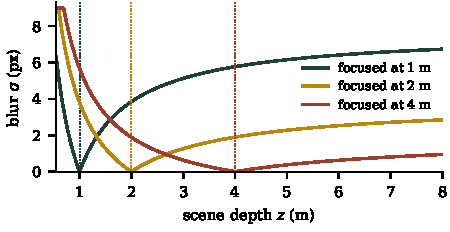
\includegraphics[width=\linewidth]{figures/blur_curve.pdf}
\captext{Fig.~1. Simulated blur at three focus distances: 25\,mm lens, f/2, focal length 1,200 pixels. The Gaussian approximation is capped at 9 pixels.}
\end{minipage}
\end{proposalbox}

\newpage
\begin{proposalbox}{Proposed Method}
We will use the published Depth Anything V2 weights without retraining and implement a classical focus baseline using the modified Laplacian [7]. At each pixel, the baseline measures sharpness across the stack and interpolates around the maximum. Calibrated focus distances give a depth estimate $z_F$. Flat or ambiguous focus curves receive low confidence $w\in[0,1]$.

\begin{center}
\begin{tikzpicture}[font=\small,box/.style={draw=Primary!70!black,fill=white,rounded corners=1mm,minimum height=10mm,text width=30mm,align=center,inner sep=3pt},arr/.style={-{Stealth[length=1.7mm]},draw=Primary,semithick}]
\node[box] (rgb) at (0,0) {Reference image};
\node[box] (net) at (3.8,0) {Depth Anything V2\\relative depth $\hat d$};
\node[box] (stack) at (0,-1.4) {Focal stack};
\node[box] (focus) at (3.8,-1.4) {Focus estimate $z_F$\\and confidence $w$};
\node[box,fill=Primary!10] (fit) at (7.6,-0.7) {Scale fitting and\\depth refinement};
\draw[arr] (rgb)--(net);
\draw[arr] (stack)--(focus);
\draw[arr] (net.east)--(fit.west);
\draw[arr] (focus.east)--(fit.west);
\end{tikzpicture}
\end{center}
\captext{Fig.~2. Proposed combination of learned relative depth and focus measurements.}

The proposed extension fits an affine transformation of the network's inverse-depth output and a local correction $r$:
\[
q(\mathbf{x})=s\hat d(\mathbf{x})+t+r(\mathbf{x}),\qquad z(\mathbf{x})=q(\mathbf{x})^{-1}.
\]
We fit reliable focus estimates with a Huber loss $\rho$ and regularize the correction:
\[
\begin{aligned}
\min_{s,t,r}\;&\sum_{\mathbf{x}}w(\mathbf{x})\rho\!\left(q(\mathbf{x})-z_F(\mathbf{x})^{-1}\right)
+\lambda\sum_{\mathbf{x}}\|\nabla r(\mathbf{x})\|^2
+\mu\sum_{\mathbf{x}}r(\mathbf{x})^2,\\
& q(\mathbf{x})\geq\epsilon>0,\qquad \lambda,\mu>0.
\end{aligned}
\]
We first fit $s,t$ with $r=0$, then allow local corrections. The two penalties discourage abrupt or large changes where focus measurements are weak. If the stack contains insufficient reliable depth variation to fit scale, the output remains relative depth and is marked uncalibrated.

This design lets us test global scale fitting separately from local refinement. It may improve on either baseline when their errors differ, but learned predictions can also fail on textureless surfaces or unfamiliar objects. The evaluation will include these cases.
\end{proposalbox}

\begin{proposalbox}{Preliminary Experiment}
A prototype renders ten focus settings from 0.9 to 7\,m using a layered Gaussian-blur model. The synthetic scene contains a textured backdrop, a painting at 1.1\,m, and a plain card at 3\,m.
\begin{center}
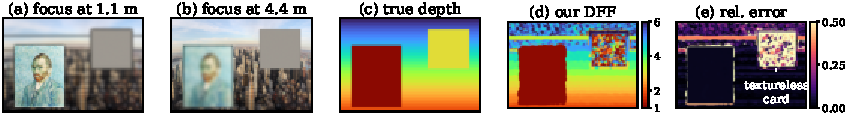
\includegraphics[width=\linewidth]{figures/dff_preliminary.pdf}
\end{center}
\captext{Fig.~3. Rendered frames, assigned depth, focus estimate, and relative error. Depth spans 1--6\,m; the error display is capped at 0.5. Textures use the HW1 image assets.}

The focus estimate is unreliable on the plain card and near depth boundaries. This experiment checks the classical baseline; the learned model and proposed refinement have not yet been evaluated.
\end{proposalbox}

\newpage
\fontsize{10.5}{12.2}\selectfont
\begin{proposalbox}{Evaluation}
We will evaluate the single-image baseline on the standard 654-image NYU-Depth v2 test set [8]. Refinement experiments require focal stacks, so we will use rendered scenes and DDFF 12-Scene [5], subject to verification of its available labels, calibration, and depth units. We will separate tuning and evaluation scenes. Results will be reported in meters only where calibration supports that conversion. Phone captures are optional qualitative examples.

\begin{tabularx}{\linewidth}{@{}p{0.30\linewidth}X@{}}
\toprule
\textbf{Method} & \textbf{Purpose}\\
\midrule
Aligned DA-V2 & Reference for shape accuracy after fitting scale and shift to ground truth.\\
Focus baseline & Depth recovered from the focal stack alone.\\
DA-V2 + scale fit & Calibration from focus measurements with $r=0$.\\
Full refinement & Effect of adding local depth corrections.\\
\bottomrule
\end{tabularx}
\par\smallskip
We will report AbsRel, RMSE, and $\delta_1$, the fraction of valid pixels satisfying $\max(z/z_{\rm gt},z_{\rm gt}/z)<1.25$. Metric predictions will be scored without ground-truth alignment; aligned scores will be reported separately. Runtime, rejected scale fits, and errors in low- and high-texture regions will also be recorded. Texture groups will use a fixed image-gradient rule selected before evaluation.

Ablations will vary confidence weighting, local corrections, regularization, and stack size (2, 3, 5, or 10 frames). All comparisons will use the same scenes, valid masks, and depth ranges. We will assess whether refinement reduces unaligned depth error relative to both the focus baseline and the scale-only fit, and report per-scene failures alongside aggregate results.
\end{proposalbox}

\begin{proposalbox}{Timeline}
\begin{tabularx}{\linewidth}{@{}p{0.23\linewidth}X@{}}
\toprule
\textbf{Dates} & \textbf{Planned work}\\
\midrule
Sep 30--Oct 9 & Run DA-V2, verify dataset access and calibration, and produce initial baseline results.\\
Oct 10--20 & Complete the focus baseline and analyze synthetic and available real stacks.\\
Oct 21--29 & Finalize baseline comparisons and write the midterm report (Oct 29).\\
Oct 30--Nov 13 & Implement scale fitting and refinement; run ablations.\\
Nov 14--24 & Complete held-out evaluation and prepare the project webpage.\\
Nov 25--Dec 10 & Prepare the Dec 1--10 presentation; finalize code and webpage by Dec 10.\\
\bottomrule
\end{tabularx}
\par\smallskip
The final deliverables are the baseline implementations, comparison tables, depth and error maps, and project webpage. If refinement does not improve accuracy, we will document its limitations and the conditions under which focus measurements are useful.
\end{proposalbox}

\begin{proposalbox}{References}
\begin{multicols}{2}
\fontsize{8}{9.5}\selectfont
\begin{enumerate}[label={[\arabic*]},leftmargin=1.7em,itemsep=2pt,topsep=0pt]
\item R. Ranftl et al. Towards Robust Monocular Depth Estimation: Mixing Datasets for Zero-Shot Cross-Dataset Transfer. \emph{TPAMI}, 2022.
\item L. Yang et al. Depth Anything V2. \emph{NeurIPS}, 2024.
\item S. F. Bhat et al. ZoeDepth: Zero-shot Transfer by Combining Relative and Metric Depth. \emph{arXiv:2302.12288}, 2023.
\item A. P. Pentland. A New Sense for Depth of Field. \emph{TPAMI}, 1987.
\item C. Hazirbas et al. Deep Depth From Focus. \emph{ACCV}, 2018.
\item M. Maximov, K. Galim, L. Leal-Taix\'e. Focus on Defocus: Bridging the Synthetic to Real Domain Gap for Depth Estimation. \emph{CVPR}, 2020.
\item S. K. Nayar and Y. Nakagawa. Shape from Focus. \emph{TPAMI}, 1994.
\item N. Silberman et al. Indoor Segmentation and Support Inference from RGBD Images. \emph{ECCV}, 2012.
\end{enumerate}
\end{multicols}
\end{proposalbox}
\end{document}
